\chapter[supplementary material: a retrospective study on machine learning-assisted stroke recognition for medical helpline calls]{Supplementary Material for: A Retrospective Study on Machine Learning-Assisted Stroke Recognition for Medical Helpline Calls}
\label{app:supplementary-retrospective}
\ifthenelse{\equal{\skipappendices}{true}}{}{

\section{Data flow digram}
In \cref{fig_retrospective:data_flowchart} we present an overview of the data flow from the initial data sources to the final stroke dataset.

\begin{sidewaysfigure}
    \centering
    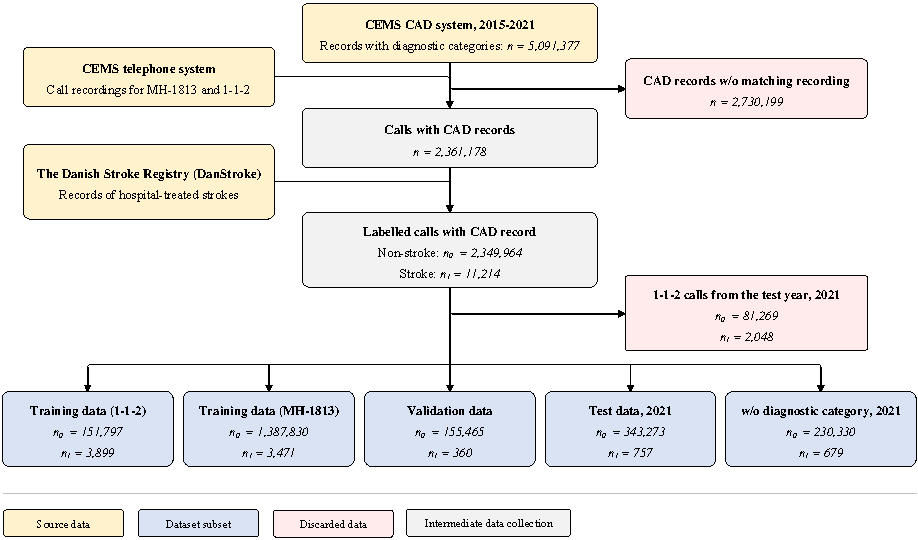
\includegraphics[width=0.8\textwidth]{paper_retrospective/data_flowchart.pdf}
    \caption[Overview of data flow from the initial data sources to the final stroke dataset.]{Overview of data flow from the initial data sources to the final stroke dataset.}
    \label{fig_retrospective:data_flowchart}
\end{sidewaysfigure}


\section{Machine learning pipeline}

\subsection{Model training}

We used stochastic gradient descent on mini-batches of data to train the stroke classification model. We used the Adam (adaptive moment estimation) optimisation algorithm and ensured an equal number of stroke positives and negatives in each batch by stratifying the class labels during sampling. We saved the model parameters after each epoch if the maximum F1-score (across all possible thresholds) improved in the validation dataset. We used the latest saved parameters as the final result of the run.

\subsection{Hyperparameters}\label{sec_retrospective:hyperparameters}

The selection of hyperparameters followed a simple two-stage process using validation data (table A1). First, a manual search was conducted by running different model configurations with varying numbers of epochs, updates per epoch, batch sizes, vectoriser types, and hyperparameters. Subsequently, a structured grid search was performed to further tune a subset of these hyperparameters.

\begin{table}
    \centering
    \caption{Overview of hyperparameters for training text classification models.}
    \label{tab_retrospective:tableA1-hyperparameters}
    \resizebox*{0.98\textwidth}{!}{%
    \begin{tabular}{l|l|l}
        \toprule

        Name & Chosen value & Grid search range \\

        \midrule

        \multicolumn{3}{c}{\emph{Determined from initial heuristic, manual hyperparameter search on validation fold}}\\

        \midrule

        Epochs & 30 & - \\
        Parameter updates per epoch & 500 & - \\
        Batch size & 128 & - \\
        Batch sampling & Label stratified (balanced) & - \\
        Type of text vectoriser & Count vectorisation & - \\
        Size of bag-of-words vector & 10,000 & - \\
        Optimisation algorithm & Adam $(\beta_1=0.9, \beta_2=0.999)$ & - \\
        Learning rate schedule & Cosine annealing from start & - \\

        \midrule

        \multicolumn{3}{c}{\emph{Determined from grid search on validation fold}} \\ 

        \midrule

        Learning rate start & 0.0003 & \{0.003, 0.0003\} \\
        Learning rate end & 0.0003 & \{0.0003, 0.00003, 0.000003\} \\
        Model input dropout & 0.50 & \{0.25, 0.50\} \\
        Model dropout & 0.25 & \{0.25, 0.50\} \\
        Model configuration & [256, 128, 64, 32, 16] & \{[64, 32, 16], [256, 128, 64, 32, 16]\} \\

        \bottomrule
    \end{tabular}%
    \vspace{-2mm}
    }
\end{table}


\paragraph{Bag-of-words selection}

Each transcript was transformed into a fixed-size bag-of-words vector to serve as input for the classification model. These vectors encode the occurrence of words and character n-grams within a fixed vocabulary. We selected vocabulary by first computing the χ2-statistics for all word uni-and bi-grams and character three-, four-, and fivegrams that occurred in more than ten training calls. We then retained the M highest-scoring word n-grams and $M$ highest-scoring character n-grams, yielding $2M$ input features, where $M$ represents a tuned hyperparameter. By complementing word n-grams with character n-grams, the model can use out-of-vocabulary words not included in the word n-grams and robustly represent words misspelt by the speech recogniser. The feature vector was input into the classification model (\cref{fig_retrospective:model_sketch}).

As part of our manual hyperparameter search, we trained the models using vectorisers of different sizes. We discovered that using 5,000-word n-grams and 5,000-character n-grams (M=5,000) struck a good trade-off between size, feature quality, and model performance, yielding 10,000 bag-of-words features.

\begin{figure}[t]
    \centering
    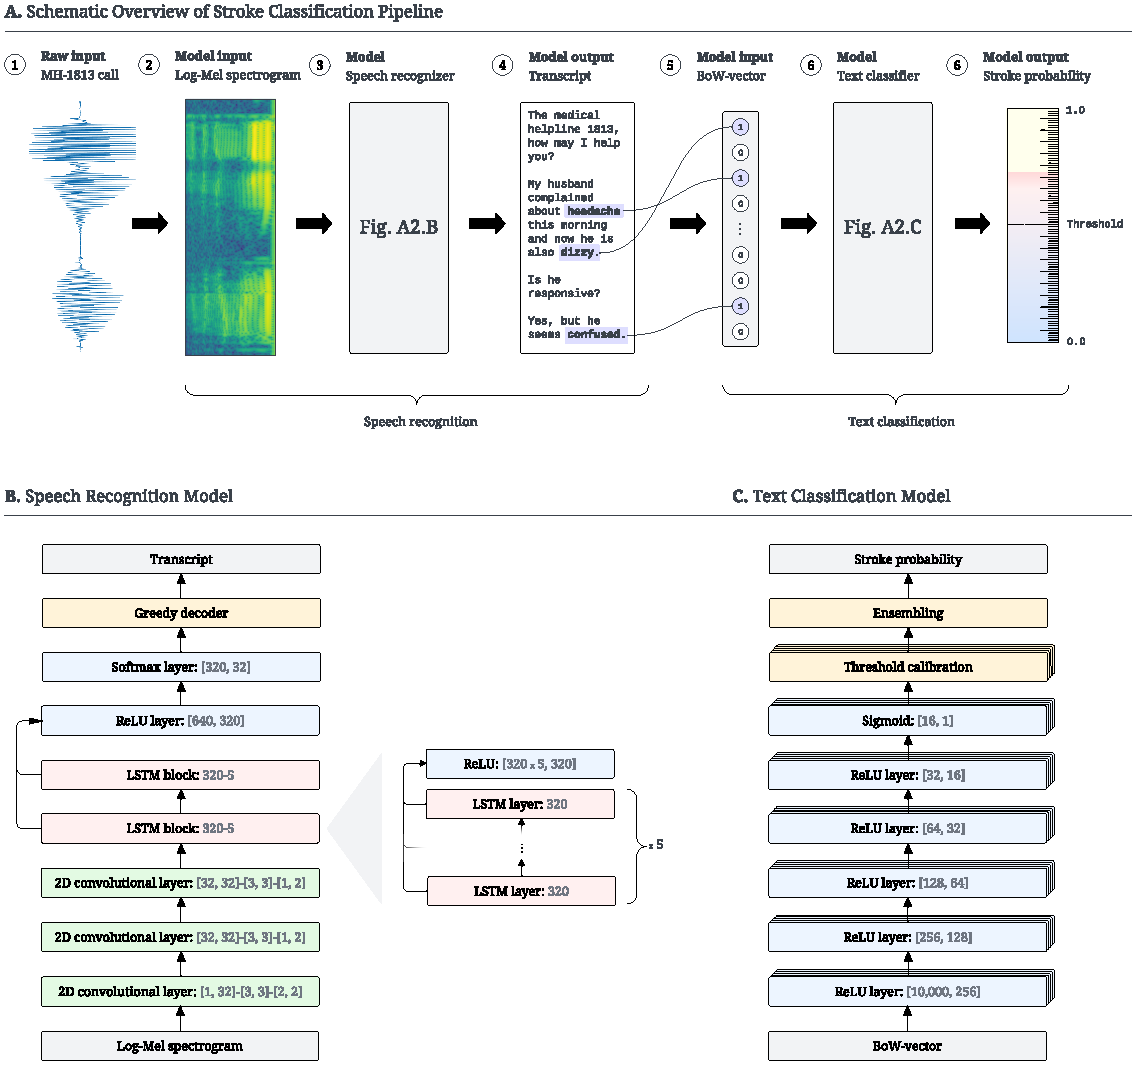
\includegraphics[width=0.95\textwidth]{paper_retrospective/model_sketch.pdf}
    \caption[Overview of machine learning pipeline for stroke recognition.]{Overview of machine learning pipeline. Panel A presents a schematic overview of the machine learning pipeline. The individual models are broken down in panels B and C. The 2D convolutional layers have parameters [input channels, output channels]-[kernel width, kernel height]-[stride width, stride height]. The long short-term memory (LSTM) blocks have parameters hidden units-number of layers. The rectified linear unit (ReLU), sigmoid, and softmax layers have parameters [input features, output features]. Joining arrows indicate the concatenation of two vector sequences along the feature dimension. The full set of model hyperparameters is listed in \cref{sec_retrospective:hyperparameters}.}
    \label{fig_retrospective:model_sketch}
\end{figure}

\subsection{Ensembling details}

A common way to combine individual classification models into an ensemble is to use a voting scheme, such as majority voting, where a combined prediction is made based on the consensus among the individual models. However, this approach makes the ensemble not have a continuous output score. This is problematic for two reasons.
%
\begin{itemize}
    \item The lack of a continuous output score prevents the evaluation of the model's performance across a continuous range of thresholds required for plotting the receiver operating characteristic and precisionrecall curves.
    \item The lack of a continuous output score deteriorates the quality of assessing the effect of different words on ensemble performances (see \cref{sec_retrospective:model_explainability}).
\end{itemize}
%
Therefore, we used a different ensemble method, which is briefly described in the main text. Herein, we provide a mathematically rigorous definition of the proposed method.

Let $z^{(n,d)}$ be the logit output of model $n$ for transcript $d$, $t^{(n)}$ be the tuned logit threshold of model $n$, and $N$ be the number of models in the ensemble. The output score $p^{(n)}$ is then given by 
%
\begin{equation}
    p^{(d)} = \frac{1}{N} \sum_{n=1}^N \sigma\left(z^{(n,d)} - t^{(n)}\right) \enspace ,
\end{equation}
%
where $\sigma(\cdot)$ is the sigmoid function (or standard logistic function). The final ensembel predction $s^{(d)}$ is then simply 
%
\begin{equation}
    s^{(d)} = I_{p^{(d)} > 0.5}\left(p^{(d)}\right) \enspace ,
\end{equation}
%
where $I_{\cdot}(\cdot)$ is the indicator function that returns 1 if the subscript condition is satisfied and 0 otherwise. 


\section{Significance testing and confidence intervals}

We used standard methods for significance testing and computing the confidence intervals. We used approximate methods owing to data size and to maintain computational feasibility \parencite{dwass_modified_1957,eden_validity_1933}

We performed \emph{paired approximate permutation} tests by pairing each observation from the first sample to a random observation from the other sample (without replacement), while keeping each observation within its original sample. This allowed us to test the significance of the observed pairings on the chosen statistics, i.e. whether a significant difference was observed in the test statistics depending on whether the call-taker or model made the prediction. We used this approach to test whether
%
\begin{itemize}
    \item the model performed better than the call-takers on the 2021 test set,
    \item including 112 training data improved the model's performance on the 2021 test set.
\end{itemize}
%
We performed \emph{independent approximate permutation} tests by randomly assigning observations to either of the two samples (without replacement) while maintaining any differences in sample size. This approach allowed us to test the significance of the observed sample assignments, i.e. whether there was a significant difference in test statistics depending on whether the predictions were assigned to the model or call-taker. We used this approach to test whether.
%
\begin{itemize}
    \item the model performed better on the 2021 test set with diagnostic categories than on the test set without diagnostic categories,
    \item the model performed better on men than women on the 2021 test set,
    \item the model performed better on the 65+ group than on the 18-64 group on the 2021 test set,
    \item the call-taker performed better on men than women on the 2021 test set,
    \item the call-taker performed better on the 65+ group than on the 18-64 group on the 2021 test set.
\end{itemize}
%
The p-values were not exact because we used approximate permutation tests. However, owing to the large dataset size and substantial number of observations, the estimated p-values had tight confidence intervals. We reported the upper bound of the 99\% confidence interval on the p-value computed as the usual binomial distribution confidence interval.
%
\begin{equation}
    \text{CI}(p) = \hat{p} \pm z \sqrt{\frac{\hat{p}(1-\hat{p})}{N}} \enspace ,
\end{equation}
%
where $N$ is the number of resamplings.

We computed \emph{bootstrapped confidence intervals} for the statistics by resampling (with replacement) the predictions made by model or call-taker on a relevant subgroup and recomputing the relevant statistics for each bootstrap sample. This process established a bootstrap distribution of the statistic that was then used to estimate the standard error and compute the confidence intervals. We computed confidence intervals using the bootstrap distribution percentiles. This method yielded reliable results because our dataset was large, and the bootstrap distribution was symmetrical and centred on the observed statistic. No observed bootstrap distributions differed significantly from normal distributions (according to Anderson-Darling and Shapiro-Wilk tests). Therefore, confidence intervals computed alternatively as studentised bootstrap intervals (t-intervals) did not differ substantially from percentile confidence intervals. This further validated our tests.

We used $N=15,000$ resamplings for permutation tests and $N=8,192$ for confidence intervals.


\section{Software}

We used Python version 3.8.10. PyTorch version 1.12.1 + cu113 was used to train the neural network models. We used SciKit-Learn (version 1.2.2) to perform bag-of-words vectorisation. We used NumPy version 1.23.5, Pandas version 1.5.3, Matplotlib version 3.7.1, and SciPy version 1.10.1 to perform data analysis, plotting, and testing.


\section{Additional results: Model performance across demographics}

When 1-1-2 data were not used for training (\cref{tab_retrospective:tableA2}), the model performed significantly better in men than in women on the test set in terms of all metrics (p < 0.0001) and significantly better on the 65+ group than on the 1864 group in terms of all metrics (p < 0.0001). As noted in the main text, both these statements were also true when 1-1-2 data were used for the training (\cref{tab_retrospective:table2-main-results}) and that including 1-1-2 data significantly improved overall performance (p < 0.0001).

Compared to the test set (\cref{tab_retrospective:table2-main-results}), model performance on the 2021 calls without diagnostic category was significantly worse in all demographic subgroups (\cref{tab_retrospective:tableA3}) in terms of all metrics (p < 0.0001), except for positive predictive value (PPV) for male (where p = 0.0056 [significant]) and for the false positive rate (FPR) on females and individuals aged 65+ years (where p = 0.213 and p = 0.362, respectively [insignificant]).

% \todo[inline]{Insert table A2 here}
\begin{table}
    \centering
    \caption{Model performance for sex and age subgroups [mean (95\% CI)] on the MH-1813 test data when 1-1-2 training data is not used for training.}
    \label{tab_retrospective:tableA2}
    \resizebox*{0.85\textwidth}{!}{%
    \begin{tabular}{l|cc|cc}
        \toprule

         & \multicolumn{4}{c|}{Model w/o 1-1-2 training data} \\
        \midrule
         & Female & Male & 18-64 years & 65+ years \\

        \midrule

        F1-score [\%] $\uparrow$ & \makecell[c]{28.7 \\ (27.8-29.6)} & \makecell[c]{36.2 \\ (35.3-37.2)} & \makecell[c]{20.5 \\ (19.5-21.5)} & \makecell[c]{39.4 \\ (38.6-40.3)} \\
        \midrule
        Sensitivity [\%] $\uparrow$ & \makecell[c]{58.2 \\ (56.7-59.9)} & \makecell[c]{62.1 \\ (60.7-63.6)} & \makecell[c]{53.0 \\ (50.9-55.0)} & \makecell[c]{63.0 \\ (61.9-64.3)} \\
        \midrule
        PPV [\%] $\uparrow$ & \makecell[c]{19.0 \\ (18.3-19.7)} & \makecell[c]{25.6 \\ (24.8-26.4)} & \makecell[c]{12.7 \\ (12.0-13.4)} & \makecell[c]{28.7 \\ (27.9-29.5)} \\
        \midrule
        \makecell[l]{FOR [\%] $\downarrow$ \\ (1 - NPV)}  & \makecell[c]{0.077 \\ (0.073-0.080)} & \makecell[c]{0.102 \\ (0.097-0.106)} & \makecell[c]{0.034 \\ (0.032-0.036)} & \makecell[c]{0.318 \\ (0.305-0.331)} \\
        \midrule
        \makecell[l]{FPR [\%] $\downarrow$ \\ (1 - specificity)} & \makecell[c]{0.45 \\ (0.446-0.463)} & \makecell[c]{0.483 \\ (0.473-0.494)} & \makecell[c]{0.264 \\ (0.258-0.270)} & \makecell[c]{1.335 \\ (1.308-1.362)} \\

        \bottomrule
    \end{tabular}%
    }
\end{table}


% \todo[inline]{Insert table A3 here}
\begin{table}
    \centering
    \caption{Model performance for sex and age subgroups [mean (95\% CI)] on the 2021 data without diagnostic category.}
    \label{tab_retrospective:tableA3}
    \resizebox*{0.85\textwidth}{!}{%
    \begin{tabular}{l|cc|cc}
        \toprule

         & \multicolumn{4}{c|}{Model} \\
        \midrule
         & Female & Male & 18-64 years & 65+ years \\

        \midrule

        F1-score [\%] $\uparrow$                                 & \makecell[c]{30.4 \\ (29.3-31.5)} & \makecell[c]{35.2 \\ (34.0-36.4)} & \makecell[c]{24.3 \\ (23.0-25.7)} & \makecell[c]{36.6 \\ (35.6-37.6)} \\
        \midrule
        Sensitivity [\%] $\uparrow$                              & \makecell[c]{44.5 \\ (42.9-46.0)} & \makecell[c]{52.8 \\ (51.1-54.4)} & \makecell[c]{45.6 \\ (43.4-47.9)} & \makecell[c]{49.2 \\ (47.9-50.5)} \\
        \midrule
        PPV [\%] $\uparrow$                                      & \makecell[c]{23.1 \\ (22.2-24.1)} & \makecell[c]{26.4 \\ (25.3-27.4)} & \makecell[c]{16.6 \\ (15.5-17.5)} & \makecell[c]{29.1 \\ (28.2-30.0)} \\
        \midrule
        \makecell[l]{FOR [\%] $\downarrow$ \\ (1 - NPV)}         & \makecell[c]{0.152 \\ (0.146-0.159)} & \makecell[c]{0.155 \\ (0.147-0.162)} & \makecell[c]{0.058 \\ (0.055-0.062)} & \makecell[c]{0.372 \\ (0.359-0.386)} \\
        \midrule
        \makecell[l]{FPR [\%] $\downarrow$ \\ (1 - specificity)} & \makecell[c]{0.404 \\ (0.394-0.414)} & \makecell[c]{0.480 \\ (0.467-0.494)} & \makecell[c]{0.246 \\ (0.239-0.254)} & \makecell[c]{0.873 \\ (0.852-0.894)} \\

        \bottomrule
    \end{tabular}%
    }
\end{table}


\section{Additional results: Model with patient age and sex as explicit inputs}

To assess the importance of patient age and sex for accurate model stroke recognition we have performed an experiment to test whether explicitly adding the age and sex of the patient as inputs to the model improves performance.

Specifically, we encode patient sex as two binary numbers which we concatenate to the bag-of-words input representation. The first has the value of 1 if the patient is female, and the second has the value of 1 if the patient is male. Neither is 1 if the patient's sex is unknown/undisclosed. Similarly, we include patient age as a 15-dimensional one-hot vector where the first value represents patients with an age below 25 and the last value represents patients with an age of 90 or above. Values in between represent 5-year intervals.

We trained the model similarly to how we performed our ablation experiments. That is, we used the hyperparameters that gave the best performance on the validation set to train 11 differently seeded versions of the model and then report mean metrics and associated CIs on the MH-1813 test data. The results are as shown in \cref{tab_retrospective:tableA4} below.

\begin{table}
    \centering
    \caption[Overall performance on MH-1813 test data for the model that also takes patient age and sex as direct inputs.]{Overall performance on MH-1813 test data for the model that also takes patient age and sex as direct inputs. We also list the original performance of call-takers and the model (w/o sex and age) from the main manuscript for ease of comparison [mean (95\% CI)].}
    \label{tab_retrospective:tableA4}
    \resizebox*{0.98\textwidth}{!}{%
    \begin{tabular}{l|ccccc}
        \toprule
        & F1-score [\%] $\uparrow$ & Sensitivity [\%] $\uparrow$ & PPV [\%] $\uparrow$ & \makecell[c]{FOR [\%] $\downarrow$ \\ (1 - NPV)} & \makecell[c]{FPR [\%] $\downarrow$ \\ (1 - specificity)} \\
        \midrule
        & \multicolumn{5}{c}{\textit{Overall}} \\
        \midrule
        
        Call-takers                             & \makecell[c]{25.8 \\ (23.7-27.9)} & \makecell[c]{52.7 \\ (49.2-56.4)} & \makecell[c]{17.1 \\ (15.5-18.6)} & \makecell[c]{0.105 \\ (0.094-0.116)} & \makecell[c]{0.565 \\ (0.539-0.590)} \\
        \midrule
        \makecell[l]{Model \\ w/o sex and age}  & \makecell[c]{35.7 \\ (35.0-36.4)} & \makecell[c]{63.0 \\ (62.0-64.1)} & \makecell[c]{24.9 \\ (24.3-25.5)} & \makecell[c]{0.082 \\ (0.079-0.085)} & \makecell[c]{0.419 \\ (0.413-0.426)} \\
        \midrule
        \makecell[l]{Model \\ w/ sex and age}   & \makecell[c]{35.8 \\ (35.1-36.5)} & \makecell[c]{64.1 \\ (63.1-65.1)} & \makecell[c]{24.9 \\ (24.3-25.4)} & \makecell[c]{0.080 \\ (0.077-0.082)} & \makecell[c]{0.427 \\ (0.421-0.434)} \\
 
        \bottomrule
    \end{tabular}%
    }
\end{table}

We note that the performance difference between the original model and the models with age and sex inputs is statistically insignificant (p > 0.05). We hypothesize this might be because information regarding the age and sex of the patient is, in many cases, already present in the transcript. Another reason might be that the patient's age and sex are less useful discriminators than other indicative factors. This latter hypothesis is supported by our occlusion analysis and \cref{tab_retrospective:table3-occlusion-analysis} where no highly ranked words directly refer to the patient's age or sex.

It is important to note that in practice the information about patient sex and age is extracted from the patient's CPR number which is typically entered by the patient themselves while queuing for MH-1813. However, at call lines in countries without similar systems in place, such information may not be readily available and cannot be incorporated as an explicit input feature. The same is the case for the 1-1-2 call line in Denmark.


\section{Additional results: Model without MH-1813 training data}
%
The ablation study in the main manuscript that examines the importance of the two different source domains (1-1-2 and MH-1813) includes only two of the three possible combinations of data sources, specifically: training on both 1-1-2 and MH-1813 data, and training only on MH-1813 excluding 1-1-2 data. For this reason, we have conducted an experiment that includes the remaining combination: training only on 1-1-2 excluding MH-1813 data.

Since the manuscript focuses on the MH-1813 line, the main purpose of experimenting with including and excluding the 1-1-2 data was to examine whether using the out-of-domain 1-1-2 data could improve stroke recognition performance of the machine learning framework on the MH-1813 data. This has interest since many prehospital call centres operate both a high acuity emergency line (like 1-1-2) and a low-acuity medical helpline (like MH-1813) which makes high-acuity data available for modelling and a potentially valuable data source. The ablation experiment performed here, on the other hand, has a different purpose. It aims to show whether a model to assist the MH-1813 helpline could be developed also in the hypothetical case of only having access to out-of-domain, high-acuity training data from 1-1-2. This prospect may be interesting for some call centres that, for instance, have only recently started operating a medical helpline, and so, do not have in-domain training data available.

We trained the models and provided the results of this experiment in \cref{tab_retrospective:tableA5} below using the same methods as in the main manuscript. We tested the significance of these results using the same statistical significance testing methods as used and described in the main manuscript.

We see that the performance of the ensemble model trained only with 1-1-2 data compared to training only with MH-1813 data was worse in terms of sensitivity and FOR (p < 0.0001), but on-par in terms of F1-score and PPV, and better in terms of FPR (p < 0.0001). Compared to training with all data, training only on 1-1-2 was worse on all metrics (p < 0.0001) except FPR, where it was better (p < 0.0001). We note that the model still performed better than the call-takers in terms of F1-score, PPV, and FPR (p < 0.0001) and was on-par in terms of sensitivity and FOR.

In summary, training on only 1-1-2 data was only somewhat worse than training on only MH-1813 data, and still outperformed call-takers to some degree. This indicates that the domain shift between different call lines, even with different acuity levels, is small enough that naive domain transfer of models works fairly well.

\begin{table}
    \centering
    \caption{Overall performance on MH-1813 test data for the original model, the model without 1-1-2 training data, and the model without 1813 training data along with call-taker performance [mean (95\% CI)].}
    \label{tab_retrospective:tableA5}
    \resizebox*{0.98\textwidth}{!}{%
    \begin{tabular}{l|ccccc}
        \toprule
        & F1-score [\%] $\uparrow$ & Sensitivity [\%] $\uparrow$ & PPV [\%] $\uparrow$ & \makecell[c]{FOR [\%] $\downarrow$ \\ (1 - NPV)} & \makecell[c]{FPR [\%] $\downarrow$ \\ (1 - specificity)} \\
        \midrule
        & \multicolumn{5}{c}{\textit{Overall}} \\
        \midrule
        
        Call-takers  & \makecell[c]{25.8 \\ (23.7-27.9)} & \makecell[c]{52,7 \\ (49,2-56.4)} & \makecell[c]{17.1 \\ (15.5-18.6)} & \makecell[c]{0.105 \\ (0.094-0.116)} & \makecell[c]{0.565 \\ (0.539-0.590)} \\
        \midrule
        Model        & \makecell[c]{35.7 \\ (35.0-36.4)} & \makecell[c]{63.0 \\ (62.0-64.1)} & \makecell[c]{24.9 \\ (24.3-25.5)} & \makecell[c]{0.082 \\ (0.079-0.085)} & \makecell[c]{0.419 \\ (0.413-0.426)} \\
        \midrule
        \makecell[l]{Model \\ w/o 1-1-2} & \makecell[c]{32.4 \\ (31.8-33.1)} & \makecell[c]{60.4 \\ (59.3-61.4)} & \makecell[c]{22.2 \\ (21.6-22.7)} & \makecell[c]{0.088 \\ (0.085-0.091)} & \makecell[c]{0.467 \\ (0.460-0.474)} \\
        \midrule
        \makecell[l]{Model \\ w/o MH-1813} & \makecell[c]{31.4 \\ (30.7-32.1)} & \makecell[c]{50.4 \\ (49.3-51.4)} & \makecell[c]{22.8 \\ (22.2-23.4)} & \makecell[c]{0.110 \\ (0.106-0.113)} & \makecell[c]{0.375 \\ (0.369-0.381)} \\

        % & \multicolumn{5}{c}{\textit{Without 1-1-2 training data (only MH-1813 data)}} \\
        % \midrule
        % Model        & \makecell[c]{32.4 \\ (31.8-33.1)} & \makecell[c]{60.4 \\ (59.3-61.4)} & \makecell[c]{22.2 \\ (21.6-22.7)} & \makecell[c]{0.088 \\ (0.085-0.091)} & \makecell[c]{0.467 \\ (0.460-0.474)} \\

        % & \multicolumn{5}{c}{\textit{Without MH-1813 training data (only 1-1-2 data)}} \\
        % \midrule
        % Model        & \makecell[c]{31.4 \\ (30.7-32.1)} & \makecell[c]{50.4 \\ (49.3-51.4)} & \makecell[c]{22.8 \\ (22.2-23.4)} & \makecell[c]{0.110 \\ (0.106-0.113)} & \makecell[c]{0.375 \\ (0.369-0.381)} \\

        \bottomrule
    \end{tabular}%
    }
\end{table}


\section{Additional results: Detailed model explainability tables}

In \cref{tab_retrospective:tableA6,tab_retrospective:tableA7} we provide detailed versions of the data presented in the model explainability section in the main manuscript. Specifically, we include the Danish word, its English translation, the rank and impact scores and the number of occurrences of each word.


% % \todo[inline]{Insert table A4 here}
\begin{table}
    \centering
    \caption{Mean impact for words with the largest positive rank score in calls predicted as stroke.}
    \label{tab_retrospective:tableA6}
    \resizebox*{\textwidth}{!}{%
    \begin{tabular}{l|llccc}
        \toprule
        \multicolumn{6}{c}{Stroke predictions, $D=1,897$} \\
        \midrule
         & \makecell{Word, $w$ \\ (\textit{Danish})} & \makecell{Translation, $w$ \\ (\textit{English})} & Rank, $r^{(w)}$ & Count, $D^{(w)}$ & \makecell{Impact, $i^{(d,w)}$ \\ mean $\pm$ std.} \\
        \midrule    
        1. & Ambulance & Ambulance & $1.000$ & $1,$680 & $0.52 \pm 0.51$ \\
        2. & Blodprop & Blood clot & $0.599$ & $89$5 & $0.51 \pm 0.58$ \\
        3. & Venstre & Left & $0.381$ & $1,$108 & $0.38 \pm 0.4$ \\
        4. & Højre & Right & $0.326$ & $1,$050 & $0.31 \pm 0.42$ \\
        5. & Dobbeltsyn & Double vision & $0.247$ & $84$ & $1.01 \pm 1.26$ \\
        6. & Ordene & The words & $0.217$ & $34$4 & $0.6 \pm 0.45$ \\
        7. & Pludselig & Suddenly & $0.142$ & $78$3 & $0.29 \pm 0.28$ \\
        8. & Arm & Arm & $0.140$ & $70$9 & $0.3 \pm 0.3$ \\
        9. & Side & Side & $0.125$ & $1,$139 & $0.23 \pm 0.21$ \\
        10. & Apopleksi & Stroke & $0.102$ & $11$7 & $0.33 \pm 0.82$ \\
        11. & Dobbelt & Double & $0.102$ & $11$3 & $0.54 \pm 0.72$ \\
        12. & Styre & Control & $0.092$ & $13$4 & $0.63 \pm 0.46$ \\
        13. & Opkald & Call & $0.067$ & $39$ & $0.18 \pm 1.22$ \\
        14. & Følelsesløs & Numb & $0.065$ & $94$ & $0.53 \pm 0.58$ \\
        15. & Minutter & Minutes & $0.064$ & $76$3 & $0.22 \pm 0.16$ \\
        16. & Talebesvær & Difficulties speaking & $0.063$ & $44$ & $0.87 \pm 0.72$ \\
        17. & Hjerneblødning & Haemorrhagic stroke & $0.060$ & $13$3 & $0.4 \pm 0.49$ \\
        18. & Hånd & Hand & $0.057$ & $29$7 & $0.28 \pm 0.31$ \\
        19. & Ambulancen & The ambulance & $0.055$ & $52$1 & $0.21 \pm 0.23$ \\
        20. & Snøvler & Slurred speech & $0.052$ & $58$ & $0.71 \pm 0.54$ \\
        21. & Blodpropper & Blood clots & $0.051$ & $22$4 & $0.27 \pm 0.36$ \\
        22. & Hurtigt & Fast & $0.048$ & $66$3 & $0.18 \pm 0.18$ \\
        23. & Udtrykke & Express & $0.044$ & $44$ & $0.59 \pm 0.74$ \\
        24. & Blodfortyndende & Blood thinner & $0.044$ & $25$9 & $0.32 \pm 0.22$ \\
        25. & Usammenhængende & Incoherent & $0.043$ & $15$ & $1.14 \pm 1.13$ \\
        26. & Skæv & Lopsided & $0.039$ & $21$1 & $0.29 \pm 0.28$ \\
        27. & Nedsat & Reduced & $0.038$ & $52$8 & $0.14 \pm 0.21$ \\
        28. & Hænger & Hangs & $0.036$ & $62$8 & $0.15 \pm 0.17$ \\
        29. & Forbigående & Transient & $0.035$ & $48$ & $0.52 \pm 0.62$ \\
        30. & Vrøvler & Not making sense & $0.033$ & $14$ & $1.13 \pm 0.89$ \\
        \bottomrule
    \end{tabular}%
    }
\end{table}

% \todo[inline]{Insert table A5 here}
\begin{table}
    \centering
    \caption{Mean impact for words with the largest negative rank score in calls predicted as non-stroke.}
    \label{tab_retrospective:tableA7}
    \resizebox*{\textwidth}{!}{%
    \begin{tabular}{l|llcrr}
        \toprule
        \multicolumn{6}{c}{Non-stroke predictions, $D=342,133$} \\
        \midrule
         & \makecell{Word, $w$ \\ (\textit{Danish})} & \makecell{Translation, $w$ \\ (\textit{English})} & Rank, $r^{(w)}$ & Count, $D^{(w)}$ & \makecell{Impact, $i^{(d,w)}$ \\ mean $\pm$ std.} \\
        \midrule    
        1. & Stivkrampe & Tetanus & $-1.000$ & $4378$ & $-19.40 \pm 10.61$ \\
        2. & Gravid & Pregnant & $-0.901$ & $8749$ & $-12.08 \pm 8.64$ \\
        3. & Skåret & Cut & $-0.772$ & $7592$ & $-11.98 \pm 8.61$ \\
        4. & Forbinding & Bandage & $-0.569$ & $4561$ & $-12.87 \pm 10.08$ \\
        5. & Amager & Amager (a location) & $-0.566$ & $23776$ & $-5.60 \pm 4.43$ \\
        6. & Klokken & O'clock & $-0.535$ & $94436$ & $-2.22 \pm 2.69$ \\
        7. & Skadestuen & The emergency room & $-0.486$ & $42809$ & $-3.72 \pm 3.23$ \\
        8. & Politiet & The police & $-0.413$ & $2903$ & $-10.73 \pm 13.77$ \\
        9. & Hævet & Swollen & $-0.388$ & $60559$ & $-2.84 \pm 2.38$ \\
        10. & Håndkøb & over the counter (otc) & $-0.372$ & $4641$ & $-11.64 \pm 6.00$ \\
        11. & Halsen & The neck & $-0.366$ & $30151$ & $-3.33 \pm 3.86$ \\
        12. & Feber & Fever & $-0.361$ & $112586$ & $-1.94 \pm 1.76$ \\
        13. & Recept & Prescription & $-0.334$ & $5450$ & $-9.87 \pm 5.82$ \\
        14. & Centimetre & Centimetre & $-0.311$ & $12026$ & $-6.01 \pm 4.39$ \\
        15. & Knæet & The knee & $-0.300$ & $8875$ & $-6.12 \pm 5.91$ \\
        16. & Apoteket & The pharmacy & $-0.267$ & $10085$ & $-6.05 \pm 4.49$ \\
        17. & Maven & The stomach & $-0.267$ & $42105$ & $-2.36 \pm 2.82$ \\
        18. & Psykiatrisk & Psychiatric & $-0.263$ & $3688$ & $-8.99 \pm 8.49$ \\
        19. & Lungebetændelse & Pneumonia & $-0.231$ & $7597$ & $-5.79 \pm 5.62$ \\
        20. & Mavesmerter & Stomach pain & $-0.209$ & $10551$ & $-5.12 \pm 4.02$ \\
        21. & Afføring & Stool & $-0.199$ & $19155$ & $-3.40 \pm 3.27$ \\
        22. & Ribbenene & The ribs & $-0.195$ & $3928$ & $-8.26 \pm 6.18$ \\
        23. & Bløde & Bleed & $-0.194$ & $10501$ & $-4.88 \pm 3.97$ \\
        24. & Bløder & Bleeding & $-0.193$ & $24313$ & $-2.90 \pm 2.93$ \\
        25. & Ribben & Ribs & $-0.189$ & $2941$ & $-8.96 \pm 7.56$ \\
        26. & Brækket & Broken & $-0.183$ & $19415$ & $-3.49 \pm 2.83$ \\
        27. & Betændelse & Inflammation & $-0.181$ & $10050$ & $-5.27 \pm 3.30$ \\
        28. & Forkølet & Common cold & $-0.161$ & $8127$ & $-5.31 \pm 3.75$ \\
        29. & Morgen & Morning or morrow & $-0.160$ & $78558$ & $-1.23 \pm 1.70$ \\
        30. & Hævelse & Swelling & $-0.159$ & $17762$ & $-3.71 \pm 2.32$ \\
        \bottomrule
    \end{tabular}%
    }
\end{table}


\section{Additional results: Fine"=tuning of Danish BERT model for stroke recognition}
%
During the preliminary experimental phase, we fine"=tuned a BERT model pre"=trained on Danish text from CommonCrawl, Wikipedia, OpenSubtitles, and other Danish online forums (available at \url{https://github.com/certainlyio/nordic_bert}). 
The model was fine"=tuned for 10,000 updates using linear learning rate warm-up (1,000 updates) and decay (9,000 updates). 
The maximum learning rate was set to $5\times 10^{-5}$ and an accumulated batch size of 128. 
The maximum sequence length of the pre"=trained model was 512 input tokens. 
To accommodate longer input sequences, which was necessary for our dataset, we concatenated several copies of the original positional embedding matrix. 
The results of the final model are presented in \cref{tab_retrospective:tableA8}. 

We see that the fine"=tuned BERT model performs slightly worse across F1-score, sensitivity, PPV and FOR (p < 0.0001), but better in terms of FPR (p < 0.0001), compared the MLP model presented in the main manuscript. As described in the discussion section, we hypothesize that the number of stroke positives was too small for these advanced models to learn more complex patterns than the MLP ensemble. In addition, the BERT model would likely benefit from pre"=training on text data from the target domain, or a domain close to it, rather than various online fora.

\begin{table}
    \centering
    \caption[Overall performance on MH-1813 test data for a fine"=tuned BERT model.]{Overall performance on MH-1813 test data for a fine"=tuned BERT model. We also list the original performance of call-takers and the ensemble model from the main manuscript for ease of comparison [mean (95\% CI)].}
    \label{tab_retrospective:tableA8}
    \resizebox*{0.98\textwidth}{!}{%
    \begin{tabular}{l|ccccc}
        \toprule
        & F1-score [\%] $\uparrow$ & Sensitivity [\%] $\uparrow$ & PPV [\%] $\uparrow$ & \makecell[c]{FOR [\%] $\downarrow$ \\ (1 - NPV)} & \makecell[c]{FPR [\%] $\downarrow$ \\ (1 - specificity)} \\
        \midrule
        & \multicolumn{5}{c}{\textit{Overall}} \\
        \midrule
        
        Call-takers                             & \makecell[c]{25.8 \\ (23.7-27.9)} & \makecell[c]{52.7 \\ (49.2-56.4)} & \makecell[c]{17.1 \\ (15.5-18.6)} & \makecell[c]{0.105 \\ (0.094-0.116)} & \makecell[c]{0.565 \\ (0.539-0.590)} \\
        \midrule
        \makecell[l]{MLP}                       & \makecell[c]{35.7 \\ (35.0-36.4)} & \makecell[c]{63.0 \\ (62.0-64.1)} & \makecell[c]{24.9 \\ (24.3-25.5)} & \makecell[c]{0.082 \\ (0.079-0.085)} & \makecell[c]{0.419 \\ (0.413-0.426)} \\
        \midrule
        \makecell[l]{BERT \\ (fine"=tuned)}      & \makecell[c]{33.8 \\ (31.5-36.2)} & \makecell[c]{57.5 \\ (53.9-60.9)} & \makecell[c]{23.9 \\ (21.9-25.9)} & \makecell[c]{0.094 \\ (0.084-0.104)} & \makecell[c]{0.403 \\ (0.381-0.424)} \\
 
        \bottomrule
    \end{tabular}%
    }
\end{table}


\section{Simulation of a prospective study on 2021 data}

\subsection{Method}

The machine learning frameworks can be deployed in different forms in clinical practice. To assess the potential outcomes of deploying this framework in a future prospective study, we performed an experiment using the 2021 test data to simulate different scenarios. Each scenario included two main variables.
%
\begin{enumerate}[label=\Roman*.]
    \item When is the model prediction presented to the call-taker?
    \item How does prediction influence the diagnostic code the call-taker assigns to the call?
\end{enumerate}
%
There are two primary options as to when the model prediction is presented (I):
%
\begin{enumerate}
    \item Notify the call-taker of potential false positive or negative stroke cases after the call ends.
    \item Notify the call-taker of potential false positive or negative stroke cases during the call.
\end{enumerate}
%
Option 1 is identical to the method used in the main study. In option 2, predictions are made during the call based only on partial transcriptions. We implemented option 2 in such a manner that the model predicted every time 50 new words were transcribed and added to the transcript. A stroke positive was triggered only when three consecutive positive predictions were made (i.e. without intermediate negative stroke predictions). In other words, the sigmoid activation of the model had to remain above 0.5 for three consecutive predictions, for example, after 150, 200, and 250 words were transcribed.

As we can only assume how call-takers are influenced by model predictions (II), precisely evaluating the hypothetical performance of call-takers when supported by a machine learning framework is impossible. Furthermore, option 2 may influence the conversation, further complicating matters. Therefore, we report the results combining the call-taker and the model under the following two assumptions:
%
\begin{enumerate}[label=\Alph*.]
    \item Call-takers change any stroke prediction from negative to positive if the model predicts a positive (call-takers mirror model positives).
    \item Call-takers change any stroke prediction from positive to negative if the model predicts a negative (call-takers mirror model negatives).
\end{enumerate}
%
By definition, method A tended to increase sensitivity and decrease PPV, whereas method B tended to decrease sensitivity and increase PPV.

We also report the results of the model itself (C). This method corresponds to call-takers mirroring the model predictions exactly. This is not feasible in practice, although technically possible, because the conversation and instructions given to patients may conflict with the actions taken by the call-taker after hanging up. Method 1.C is identical to the method employed in the main text, and we have copied the same results here for easier comparison.


\subsection{Results}

As expected (\cref{tab_retrospective:tableA9}), method 2.C (raw model predictions during calls) yielded slightly worse results than 1.C (raw model predictions after calls). Compared with method C, method A (call-takers mirror model positives) led to increased sensitivity and decreased PPV, whereas method B (call-takers mirror model negatives) led to decreased sensitivity and increased PPV, as expected. The numerical changes compared with method C are quite large because, in our simulation, the call-taker is assumed to strictly follow methods A or B without divergence.

% \todo[inline]{Insert table A6 here}
\begin{sidewaystable}
    \centering
    \caption{Overall performance of model, call-takers and simulated combinations of model and call-takers on MH-1813 test data.}
    \label{tab_retrospective:tableA9}
    \resizebox*{0.98\textwidth}{!}{%
    \begin{tabular}{c|c|cc|cc|cc}
        \toprule

        Predictor & Call-taker & \multicolumn{2}{c|}{Model} & \multicolumn{4}{c}{Call-taker supported by the model (simulated)} \\
        \midrule
        When & - & After call & During call & After call & During call & After call & During call \\
        \midrule
        Method & - & 1.C & 2.C & 1.A & 1.B & 2.A & 2.B \\
        \midrule

        \makecell[l]{F1-score [\%] $\uparrow$}                   & \makecell[c]{25.8 \\ (23.7-27.9)} & \makecell[c]{35.7 \\ (35.0-36.4)} & \makecell[c]{33.1 \\ (32.4-33.7)} & \makecell[c]{28.9 \\ (28.3-29.5)} & \makecell[c]{33.3 \\ (32.5-34.1)} & \makecell[c]{27.6 \\ (27.0-28.1)} & \makecell[c]{32.7 \\ (31.8-33.5)} \\
        \midrule
        \makecell[l]{Sensitivity [\%] $\uparrow$}                & \makecell[c]{52.7 \\ (49.2-56.4)} & \makecell[c]{63.0 \\ (62.0-64.1)} & \makecell[c]{58.7 \\ (57.7-59.8)} & \makecell[c]{72.4 \\ (71.5-73.3)} & \makecell[c]{43.4 \\ (42.3-44.5)} & \makecell[c]{72.3 \\ (71.4-73.3)} & \makecell[c]{39.1 \\ (38.1-40.1)} \\
        \midrule
        \makecell[l]{PPV [\%] $\uparrow$}                        & \makecell[c]{17.1 \\ (15.5-18.6)} & \makecell[c]{24.9 \\ (24.3-25.5)} & \makecell[c]{23.0 \\ (22.5-23.6)} & \makecell[c]{18.0 \\ (17.6-18.4)} & \makecell[c]{27.0 \\ (26.3-27.8)} & \makecell[c]{17.0 \\ (16.7-17.4)} & \makecell[c]{28.1 \\ (27.3-28.9)} \\
        \midrule
        \makecell[l]{FOR [\%] $\downarrow$ \\ (1 - NPV)}         & \makecell[c]{0.105 \\ (0.094-0.116)} & \makecell[c]{0.082 \\ (0.079-0.085)} & \makecell[c]{0.091 \\ (0.088-0.094)} & \makecell[c]{0.061 \\ (0.059-0.064)} & \makecell[c]{0.125 \\ (0.121-0.129)} & \makecell[c]{0.061 \\ (0.059-0.064)} & \makecell[c]{0.134 \\ (0.131-0.138)} \\
        \midrule
        \makecell[l]{FPR [\%] $\downarrow$ \\ (1 - specificity)} & \makecell[c]{0.565 \\ (0.539-0.590)} & \makecell[c]{0.419 \\ (0.413-0.426)} & \makecell[c]{0.432 \\ (0.426-0.439)} & \makecell[c]{0.726 \\ (0.717-0.735)} & \makecell[c]{0.258 \\ (0.253-0.263)} & \makecell[c]{0.776 \\ (0.767-0.786)} & \makecell[c]{0.221 \\ (0.216-0.226)} \\

        \bottomrule
    \end{tabular}%
    }
\end{sidewaystable}

Method 1.A (call-takers mirror model positives after a call) yields a better F1-score, sensitivity, PPV, and FOR than call-takers alone, although at the cost of a slightly higher FPR. This stands in contrast to methods 1.B, 2.A, and 2.B where either the sensitivity or the PPV is worse for the combined system than for call-takers alone. Regardless, the F1-score (harmonic mean of sensitivity and PPV) is higher for all methods of combining call-takers and model (1.A through 2.C).

These findings highlight that the implementation strategy selected for practice can substantially affect performance. Therefore, it may be possible to implement the system in a way that improves stroke recognition in practice.


\section{Research in context}

\subsection{Evidence before this study}

We searched the PubMed database for articles published in any language up to 9 May 2023 using the following terms: stroke AND (artificial intelligence OR machine learning OR deep learning) AND (EMS OR emergency medical services OR dispatch OR telephone). We identified 88 articles, none of which reported the results of machine learning-based stroke recognition during telephone calls.

One study assessed the potential impact of using speech classification software for stroke recognition by extrapolating results from a similar solution for recognising cardiac arrest. Several authors of this study co-authored the article; however, it did not report the results of an actual novel machine learning framework. The remaining articles primarily reported the use of machine learning in imaging diagnostics, stroke recognition using movement-tracking mobile devices, and the development of stroke recognition tools using other non-audio data.

\subsection{Added value of this study}

This study is the first to investigate the use of a machine learning framework for stroke recognition in medical helpline calls. The study's results can be replicated in other call lines and for other acute illnesses. A machine learning framework has been previously described for outof-hospital cardiac arrest; however, our results illustrate the feasibility of employing machine learning for detecting stroke - a more complex acute condition.

\subsection{Implications of all the available evidence}

Implementing the framework described in this study could lead to improved recognition of patients with stroke during initial contact with health services. Improving recognition would result in more patients being eligible for advanced stroke treatment and better overall outcomes owing to faster referral to a stroke unit.


\section{Research in context search term results}
The search terms stroke AND (artificial intelligence OR machine learning OR deep learning) AND (EMS OR emergency medical services OR dispatch OR telephone) yielded 88 articles in PubMed. These articles are listed below:

{\small
\begin{enumerate}
    \item Soun J.E., Chow D.S., Nagamine M. et al. "Artificial Intelligence and Acute Stroke Imaging". \textit{American Journal of Neuroradiology} (2021); 42: 2-11.
    \item Murray N.M., Unberath M., Hager G.D., Hui F.K. "Artificial Intelligence to Diagnose Ischemic Stroke and Identify Large Vessel Occlusions: A Systematic Review". \textit{Journal of Neurointerventional Surgery} (2020); 12: 156-64.
    \item Shlobin N.A., Baig A.A., Waqas M. et al. "Artificial Intelligence for Large-Vessel Occlusion Stroke: A Systematic Review". \textit{World Neurosurgery} (2022); 159: 207-20.e1.
    \item Linder S.M., Rosenfeldt A.B., Bay R.C., Sahu K., Wolf S.L., Alberts J.L. "Improving Quality of Life and Depression After Stroke Through Telerehabilitation". \textit{The American Journal of Occupational Therapy: Official Publication of the American Occupational Therapy Association} (2015); 69: 6902290020p1-10.
    \item Humphreys K., Shover C.L., Andrews C.M. et al. "Responding to the Opioid Crisis in North America and Beyond: Recommendations of the Stanford-Lancet Commission". \textit{The Lancet (London, England)} (2022); 399: 555-604.
    \item Fassbender K., Lesmeister M., Merzou F. "Prehospital Stroke Management and Mobile Stroke Units". \textit{Current Opinion in Neurology} (2023); 36: 140-6.
    \item McDonough R.V., Ospel J.M., Majoie C.B.L.M. et al. "Clinical Outcome of Patients with Mild Pre-Stroke Morbidity Following Endovascular Treatment: A HERMES Substudy". \textit{Journal of Neurointerventional Surgery} (2023); 15: 214-20.
    \item Bat-Erdene B.O., Saver J.L. "Automatic Acute Stroke Symptom Detection and Emergency Medical Systems Alerting by Mobile Health Technologies: A Review". \textit{Journal of Stroke and Cerebrovascular Diseases: The Official Journal of National Stroke Association} (2021); 30: 105826.
    \item Bonini N., Vitolo M., Imberti J.F. et al. "Mobile Health Technology in Atrial Fibrillation". \textit{Expert Review of Medical Devices} (2022); 19: 327-40.
    \item Scholz M.L., Collatz-Christensen H., Blomberg S.N.F., Boebel S., Verhoeven J., Krafft T. "Artificial Intelligence in Emergency Medical Services Dispatching: Assessing the Potential Impact of an Automatic Speech Recognition Software on Stroke Detection Taking the Capital Region of Denmark as Case in Point". \textit{Scandinavian Journal of Trauma, Resuscitation, and Emergency Medicine} (2022); 30: 36.
    \item Gupta R., Krishnam S.P., Schaefer P.W., Lev M.H., Gonzalez R.G. "An East Coast Perspective on Artificial Intelligence and Machine Learning: Part 2 - Ischemic Stroke Imaging and Triage". \textit{Neuroimaging Clinics of North America} (2020); 30: 467-78.
    \item Esbjörnsson M., Ullberg T. "Safety and Usability of Wearable Accelerometers for Stroke Detection: The STROKE ALARM PRO 1 Study". \textit{Journal of Stroke and Cerebrovascular Diseases: The Official Journal of National Stroke Association} (2022); 31: 106762.
    \item Fast L., Temuulen U., Villringer K. et al. "Machine Learning-Based Prediction of Clinical Outcomes After First-Ever Ischemic Stroke". \textit{Frontiers in Neurology} (2023); 14: 1114360.
    \item Gupta R., Krishnam S.P., Schaefer P.W., Lev M.H., Gilberto Gonzalez R. "An East Coast Perspective on Artificial Intelligence and Machine Learning: Part 1 - Hemorrhagic Stroke Imaging and Triage". \textit{Neuroimaging Clinics of North America} (2020); 30: 459-66.
    \item Cai T., Ni H., Yu M. et al. "DeepStroke: An Efficient Stroke Screening Framework for Emergency Rooms with Multimodal Adversarial Deep Learning". \textit{Medical Image Analysis} (2022); 80: 102522.
    \item Zachrison K.S., Dhand A., Schwamm L.H., Onnela J.P. "A Network Approach to Stroke Systems of Care". \textit{Circulation. Cardiovascular Quality and Outcomes} (2019); 12: e005526.
    \item O'Connell G.C., Walsh K.B., Smothers C.G. et al. "Use of Deep Artificial Neural Networks to Identify Stroke During Triage via Subtle Changes in Circulating Cell Counts". \textit{BMC Neurology} (2022); 22: 206.
    \item Yang L., Liu Q., Zhao Q., Zhu X., Wang L. "Machine Learning Is a Valid Method for Predicting Prehospital Delay After Acute Ischemic Stroke". \textit{Brain and Behavior} (2020); 10: e01794.
    \item Aldridge C.M., McDonald M.M., Wruble M. et al. "Human vs. Machine Learning-Based Detection of Facial Weakness Using Video Analysis". \textit{Frontiers in Neurology} (2022); 13: 878282.
    \item Lachance C.C., Ford C. "Portable Stroke Detection Devices for Patients with Stroke Symptoms: A Review of Diagnostic Accuracy and Cost-Effectiveness". \textit{Canadian Agency for Drugs and Technologies in Health} (2019).
    \item Fardoun H.M., Mashat A.S. "Methodologies, Models, and Algorithms for Patients Rehabilitation". \textit{Methods of Information in Medicine} (2016); 55: 60-4.
    \item Wibring K., Magnusson C., Axelsson C., Lundgren P., Herlitz J., Andersson Hagiwara M. "Towards Definitions of Time-Sensitive Conditions in Prehospital Care". \textit{Scandinavian Journal of Trauma, Resuscitation, and Emergency Medicine} (2020); 28: 7.
    \item Mayampurath A., Parnianpour Z., Richards C.T. et al. "Improving Prehospital Stroke Diagnosis Using Natural Language Processing of Paramedic Reports". \textit{Stroke} (2021); 52: 2676-9.
    \item Morey J.R., Zhang X., Yaeger K.A. et al. "Real-World Experience with Artificial Intelligence-Based Triage in Transferred Large Vessel Occlusion Stroke Patients". \textit{Cerebrovascular Diseases (Basel, Switzerland)} (2021); 50: 450-5.
    \item Sung S.F., Hung L.C., Hu Y.H. "Developing a Stroke Alert Trigger for Clinical Decision Support at Emergency Triage Using Machine Learning". \textit{International Journal of Medical Informatics} (2021); 152: 104505.
    \item Zhang Z., Zhou D., Zhang J. et al. "Multilayer Perceptron-Based Prediction of Stroke Mimics in Prehospital Triage". \textit{Scientific Reports} (2022); 12: 17994.
    \item Park E., Lee K., Han T., Nam H.S. "Automatic Grading of Stroke Symptoms for Rapid Assessment Using Optimized Machine Learning and 4-Limb Kinematics: Clinical Validation Study". \textit{Journal of Medical Internet Research} (2020); 22: e20641.
    \item Chen M., Tan X., Padman R. "A Machine Learning Approach to Support Urgent Stroke Triage Using Administrative Data and Social Determinants of Health at Hospital Presentation: Retrospective Study". \textit{Journal of Medical Internet Research} (2023); 25: e36477.
    \item Uchida K., Kouno J., Yoshimura S. et al. "Development of Machine Learning Models to Predict Probabilities and Types of Stroke at Prehospital Stage: The Japan Urgent Stroke Triage Score Using Machine Learning (JUST-ML)". \textit{Translational Stroke Research} (2022); 13: 370-81.
    \item Finck T., Schinz D., Grundl L. et al. "Automated Detection of Ischemic Stroke and Subsequent Patient Triage in Routinely Acquired Head CT". \textit{Clinical Neuroradiology} (2022); 32: 419-26.
    \item Sangal R.B., Fodeh S., Taylor A. et al. "Identification of Patients with Nontraumatic Intracranial Hemorrhage Using Administrative Claims Data". \textit{Journal of Stroke and Cerebrovascular Diseases: The Official Journal of National Stroke Association} (2020); 29: 105306.
    \item Adedinsewo D., Carter R.E., Attia Z. et al. "Artificial Intelligence-Enabled ECG Algorithm to Identify Patients with Left Ventricular Systolic Dysfunction Presenting to the Emergency Department with Dyspnea". \textit{Circulation. Arrhythmia and Electrophysiology} (2020); 13: e008437.
    \item Liu L., Yu B., Han M., Yuan S., Wang N. "Mild Cognitive Impairment Understanding: An Empirical Study by Data-Driven Approach". \textit{BMC Bioinformatics} (2019); 20: 481.
    \item Hayashi Y., Shimada T., Hattori N. et al. "A Prehospital Diagnostic Algorithm for Strokes Using Machine Learning: A Prospective Observational Study". \textit{Scientific Reports} (2021); 11: 20519.
    \item Grant L., Joo P., Nemnom M.J., Thiruganasambandamoorthy V. "Machine Learning Versus Traditional Methods for the Development of Risk Stratification Scores: A Case Study Using Original Canadian Syncope Risk Score Data". \textit{Internal and Emergency Medicine} (2022); 17: 1145-53.
    \item van Meenen L.C.C., van Stigt M.N., Marquering H.A. et al. "Detection of Large Vessel Occlusion Stroke with Electroencephalography in the Emergency Room: First Results of the ELECTRA-STROKE Study". \textit{Journal of Neurology} (2022); 269: 2030-8.
    \item van Meenen L.C.C., den Hartog S.J., Groot A.E. et al. "Relationship Between Primary Stroke Center Volume and Time to Endovascular Thrombectomy in Acute Ischemic Stroke". \textit{European Journal of Neurology} (2021); 28: 4031-8.
    \item Chien H.C., Yang T.L., Juang W.C., Chen Y.A., Li Y.J., Chen C.Y. "Pilot Report for Intracranial Hemorrhage Detection with Deep Learning Implanted Head Computed Tomography Images at Emergency Department". \textit{Journal of Medical Systems} (2022); 46: 49.
    \item Huo D., Leppert M., Pollard R. et al. "Large Vessel Occlusion Prediction in the Emergency Department with National Institutes of Health Stroke Scale Components: A Machine Learning Approach". \textit{Journal of Stroke and Cerebrovascular Diseases: The Official Journal of National Stroke Association} (2021); 30: 106030.
    \item Wu M.R., Chen Y.T., Li Z.X. et al. "Dysphagia Screening and Pneumonia After Subarachnoid Hemorrhage: Findings from the Chinese Stroke Center Alliance". \textit{CNS Neuroscience \& Therapeutics} (2022); 28: 913-21.
    \item Bacchi S., Oakden-Rayner L., Zerner T., Kleinig T., Patel S., Jannes J. "Deep Learning Natural Language Processing Successfully Predicts the Cerebrovascular Cause of Transient Ischemic Attack-Like Presentations". \textit{Stroke} (2019); 50: 758-60.
    \item Heldt F.S., Vizcaychipi M.P., Peacock S. et al. "Early Risk Assessment for COVID-19 Patients from Emergency Department Data Using Machine Learning". \textit{Scientific Reports} (2021); 11: 4200.
    \item Lu Z., Xiong Y., Yang K. et al. "What Predicts Large Vessel Occlusion in Mild Stroke Patients". \textit{BMC Neurology} (2023); 23: 29.
    \item Marijon E., Garcia R., Narayanan K., Karam N., Jouven X. "Fighting Against Sudden Cardiac Death: Need for a Paradigm Shift-Adding Near-Term Prevention and Pre-Emptive Action to Long-Term Prevention". \textit{European Heart Journal} (2022); 43: 1457-64.
    \item You J., Yu P.L.H., Tsang A.C.O. et al. "3D Dissimilar-Siamese-U-Net for Hyperdense Middle Cerebral Artery Sign Segmentation". \textit{Computerized Medical Imaging and Graphics: The Official Journal of the Computerized Medical Imaging Society} (2021); 90: 101898.
    \item Moral-Munoz J.A., Zhang W., Cobo M.J., Herrera-Viedma E., Kaber D.B. "Smartphone-Based Systems for Physical Rehabilitation Applications: A Systematic Review". \textit{Assistive Technology: The Official Journal of RESNA} (2021); 33: 223-36.
    \item Salman O.H., Aal-Nouman M.I., Taha Z.K., Alsabah M.Q., Hussein Y.S., Abdelkareem Z.A. "Formulating Multi-Diseases Dataset for Identifying, Triaging, and Prioritizing Patients to Multi-Medical Emergency Levels: Simulated Dataset Accompanied with Codes". \textit{Data in Brief} (2021); 34: 106576.
    \item Desai A., Zumbo A., Giordano M. et al. "Word2Vec Word Embedding-Based Artificial Intelligence Model in the Triage of Patients with Suspected Diagnosis of Major Ischemic Stroke: A Feasibility Study". \textit{International Journal of Environmental Research and Public Health} (2022); 19: 15295.
    \item Rinkel L.A., Prick J.C.M., Slot R.E.R. et al. "Impact of the COVID-19 Outbreak on Acute Stroke Care". \textit{Journal of Neurology} (2021); 268: 403-8.
    \item Chilamkurthy S., Ghosh R., Tanamala S. et al. "Deep Learning Algorithms for Detection of Critical Findings in Head CT Scans: A Retrospective Study". \textit{The Lancet (London, England)} (2018); 392: 2388-96.
    \item Kramer N.M., Demaerschalk B.M. "A Novel Application of Teleneurology: Robotic Telepresence in Supervision of Neurology Trainees". \textit{Telemedicine Journal and E-Health: The Official Journal of the American Telemedicine Association} (2014); 20: 1087-92.
    \item Yadav K., Sarioglu E., Choi H.A., Cartwright W.B., Hinds P.S., Chamberlain J.M. "Automated Outcome Classification of Computed Tomography Imaging Reports for Pediatric Traumatic Brain Injury". \textit{Academic Emergency Medicine: Official Journal of the Society for Academic Emergency Medicine} (2016); 23: 171-8.
    \item van Meenen L.C.C., Riedijk F., Stolp J. et al. "Pre- and Interhospital Workflow Times for Patients with Large Vessel Occlusion Stroke Transferred for Endovascular Thrombectomy". \textit{Frontiers in Neurology} (2021); 12: 730250.
    \item Saberi-Movahed F., Mohammadifard M., Mehrpooya A. et al. "Decoding Clinical Biomarker Space of COVID-19: Exploring Matrix Factorization-Based Feature Selection Methods". \textit{Computers in Biology and Medicine} (2022); 146: 105426.
    \item Shimada T., Matsubara K., Koyama D. et al. "Development of Evaluation System for Cerebral Artery Occlusion in Emergency Medical Services: Noninvasive Measurement and Utilization of Pulse Waves". \textit{Scientific Reports} (2023); 13: 3339.
    \item Gil-Jardiné C., Chenais G., Pradeau C. et al. "Trends in Reasons for Emergency Calls During the COVID-19 Crisis in the Department of Gironde, France Using Artificial Neural Network for Natural Language Classification". \textit{Scandinavian Journal of Trauma, Resuscitation and Emergency Medicine} (2021); 29: 55.
    \item Santala O.E., Lipponen J.A., Jäntti H. et al. "Continuous mHealth Patch Monitoring for the Algorithm-Based Detection of Atrial Fibrillation: Feasibility and Diagnostic Accuracy Study". \textit{JMIR Cardio} (2022); 6: e31230.
    \item O'Brien M.K., Shawen N., Mummidisetty C.K. et al. "Activity Recognition for Persons with Stroke Using Mobile Phone Technology: Toward Improved Performance in a Home Setting". \textit{Journal of Medical Internet Research} (2017); 19: e184.
    \item Bateman R.M., Sharpe M.D., Jagger J.E. et al. "36th International Symposium on Intensive Care and Emergency Medicine: Brussels, Belgium. 15-18 March 2016". \textit{Critical Care (London, England)} (2016); 20: 94.
    \item Modica C.M., Johnson B.R., Zalewski C. et al. "Hearing Loss and Irritability Reporting Without Vestibular Differences in Explosive Breaching Professionals". \textit{Frontiers in Neurology} (2020); 11: 588377.
    \item Palmcrantz S., Plantin J., Borg J. "Factors Affecting the Usability of an Assistive Soft Robotic Glove after Stroke or Multiple Sclerosis". \textit{Journal of Rehabilitation Medicine} (2020); 52: jrm00027.
    \item Mitsopoulos K., Fiska V., Tagaras K. et al. "NeuroSuitUp: System Architecture and Validation of a Motor Rehabilitation Wearable Robotics and Serious Game Platform". \textit{Sensors (Basel, Switzerland)} (2023); 23: 3281.
    \item Meng G., Tan Y., Fang M., Yang H., Liu X., Zhao Y. "Meteorological Factors Related to Emergency Admission of Elderly Stroke Patients in Shanghai: Analysis with a Multilayer Perceptron Neural Network". \textit{Medical Science Monitor: International Medical Journal of Experimental and Clinical Research} (2015); 21: 3600-7.
    \item Iglesias J.E., Schleicher R., Laguna S. et al. "Quantitative Brain Morphometry of Portable Low-Field-Strength MRI Using Super-Resolution Machine Learning". \textit{Radiology} (2023); 306: e220522.
    \item Lai F. "Stroke Networks Based on Robotic Telepresence". \textit{Journal of Telemedicine and Telecare} (2009); 15: 135-6.
    \item Kim D., Oh J., Im H., Yoon M., Park J., Lee J. "Automatic Classification of the Korean Triage Acuity Scale in Simulated Emergency Rooms Using Speech Recognition and Natural Language Processing: A Proof of Concept Study". \textit{Journal of Korean Medical Science} (2021); 36: e175.
    \item Jonsson A., Binongo J., Patel P. et al. "Mastering the Learning Curve for Robotic-Assisted Coronary Artery Bypass Surgery". \textit{The Annals of Thoracic Surgery} (2023); 115: 1118-25.
    \item Knowlton S.M., Sencan I., Aytar Y. et al. "Sickle Cell Detection Using a Smartphone". \textit{Scientific Reports} (2015); 5: 15022.
    \item Che F., Liu Y., Gong X. et al. "Extracranial Carotid Plaque Hemorrhage Is Independently Associated with Poor 3-Month Functional Outcome after Acute Ischemic Stroke-A Prospective Cohort Study". \textit{Frontiers in Neurology} (2021); 12: 780436.
    \item Boers A.M.M., Jansen I.G.H., Brown S. et al. "Mediation of the Relationship Between Endovascular Therapy and Functional Outcome by Follow-Up Infarct Volume in Patients with Acute Ischemic Stroke". \textit{JAMA Neurology} (2019); 76: 194-202.
    \item Stone J.R., Avants B.B., Tustison N.J. et al. "Functional and Structural Neuroimaging Correlates of Repetitive Low-Level Blast Exposure in Career Breachers". \textit{Journal of Neurotrauma} (2020); 37: 2468-81.
    \item Rickards C.A., Vyas N., Ryan K.L. et al. "Are You Bleeding? Validation of a Machine-Learning Algorithm for Determination of Blood Volume Status: Application to Remote Triage". \textit{Journal of Applied Physiology (Bethesda, Md. : 1985)} (2014); 116: 486-94.
    \item Edwards K.A., Greer K., Leete J. et al. "Neuronally-Derived Tau Is Increased in Experienced Breachers and Is Associated with Neurobehavioral Symptoms". \textit{Scientific Reports} (2021); 11: 19527.
    \item Cheng A.L., Liu J., Bravo S., Miller J.C., Pahlevan N.M. "Screening Left Ventricular Systolic Dysfunction in Children Using Intrinsic Frequencies of Carotid Pressure Waveforms Measured by a Novel Smartphone-Based Device". \textit{Physiological Measurement} (2023); 44.
    \item Grunwald I.Q., Kulikovski J., Reith W. et al. "Collateral Automation for Triage in Stroke: Evaluating Automated Scoring of Collaterals in Acute Stroke on Computed Tomography Scans". \textit{Cerebrovascular Diseases (Basel, Switzerland)} (2019); 47: 217-22.
    \item Hyakutake K., Morishita T., Saita K. et al. "Effects of Home-Based Robotic Therapy Involving the Single-Joint Hybrid Assistive Limb Robotic Suit in the Chronic Phase of Stroke: A Pilot Study". \textit{BioMed Research International} (2019); 2019: 5462694.
    \item Murray C., Ortiz E., Kubin C. "Application of a Robot for Critical Care Rounding in Small Rural Hospitals". \textit{Critical Care Nursing Clinics of North America} (2014); 26: 477-85.
    \item Edwards K.A., Leete J.J., Tschiffely A.E. et al. "Blast Exposure Results in Tau and Neurofilament Light Chain Changes in Peripheral Blood". \textit{Brain Injury} (2020); 34: 1213-21.
    \item Oresko J.J., Duschl H., Cheng A.C. "A Wearable Smartphone-Based Platform for Real-Time Cardiovascular Disease Detection via Electrocardiogram Processing". \textit{IEEE Transactions on Information Technology in Biomedicine: A Publication of the IEEE Engineering in Medicine and Biology Society} (2010); 14: 734-40.
    \item Alcoceba-Herrero I., Coco-Martín M.B., Leal-Vega L. et al. "Randomized Controlled Trial Evaluating the Benefit of a Novel Clinical Decision Support System for the Management of COVID-19 Patients in Home Quarantine: A Study Protocol". \textit{International Journal of Environmental Research and Public Health} (2023); 20: 2300.
    \item van Meenen L.C.C., Groot A.E., Venema E. et al. "Interhospital Transfer vs. Direct Presentation of Patients with a Large Vessel Occlusion Not Eligible for IV Thrombolysis". \textit{Journal of Neurology} (2020); 267: 2142-50.
    \item Forghani R., Gupta R. "Case of the Season: Artificial Intelligence in Clinical Practice-Large Vessel Occlusion Triage in Stroke Imaging". \textit{Seminars in Roentgenology} (2023); 58: 147-51.
    \item Jabbour P., Gonzalez L.F., Tjoumakaris S., Randazzo C., Rosenwasser R. "Stroke in the Robotic Era". \textit{World Neurosurgery} (2010); 73: 603-4.
    \item Larkin H. "On the Spot When Doc Is Not". \textit{Hospitals \& Health Networks} (2008); 82: 41-2.
    \item Jiang Y., Guarino P., Ma S. et al. "Bayesian Accrual Prediction for Interim Review of Clinical Studies: Open Source R Package and Smartphone Application". \textit{Trials} (2016); 17: 336.
    \item Lee J.H., Oh B.J., Ahn J.Y. et al. "Effectiveness of Automatic Acute Stroke Alert System Based on UMLS Mapped Local Terminology Codes at Emergency Department". \textit{AMIA ... Annual Symposium Proceedings. AMIA Symposium} (2008); 1018.
    \item "Robot Saves ED Stroke Patients, Addresses Subspecialist Shortage". \textit{ED Management: The Monthly Update on Emergency Department Management} (2011); 23: 13-5.
    \item Nagy Z., Simon P., Sipos E., Kozmann G. "The Main Elements of the Information System of the National Stroke Program (Smart Card - Telecommunication - Knowledge Bases)". \textit{Medinfo. MEDINFO} (1995); 8 Pt 2: 1496-9.
\end{enumerate}
}
}